\documentclass[12pt]{exam}
\usepackage{epsfig}
\usepackage[usenames,dvipsnames,svgnames,table]{xcolor}
\usepackage{listings}
\usepackage{color}
\usepackage{float}
\usepackage{bookmark}

% Must be last
\usepackage{hyperref}

\hypersetup{
    colorlinks=true,
    linkcolor=blue,
    filecolor=magenta,
    urlcolor=blue,
}

\newcommand{\note}[1]{\marginpar{\LARGE $\spadesuit$}
      $\spadesuit$ {\bf #1} $\spadesuit$}
      
\lstdefinestyle{error}{
  emptylines=1,
  breaklines=true,
  basicstyle=\ttfamily\color{red}
}

\lstdefinestyle{command}{
  emptylines=1,
  breaklines=true,
  basicstyle=\ttfamily\color{black}
}


\pagestyle{headandfoot}
\firstpageheader{}{}{}
\runningheader{CPSC 314}{Assignment 1}{Due Sep 27, 2021}
\setlength{\parindent}{0pt}
\begin{document}

\title{CPSC 314\\
  Assignment 1: Hello Armadillo! Introduction to Three.js, WebGL, and Shaders}
\date{Due 11:59PM, September 27, 2021}

\maketitle 

\section{Introduction}

The main goals of this assignment are to setup your graphics
development environment, including checking your browser
compatibility, setting up a local server, and an initial
exploration of the three.js library, along with the uses of vertex and fragment shaders. For this exploration you
will be using a template provided by the instructor, including shader
code ({\tt .glsl} files in the {\tt glsl/} folder).

Your main work will be to develop a high level understanding of how
the code works, to modify or write shaders, and to use
rudimentary communication between the JavaScript program and the
shaders.  Some of the details of what is going on in the rest of the
code will only become clear a bit later in the course.  You are of
course welcome to take a peek now, especially for the last part of the
assignment.  Some of the concepts are explained in Appendix A of your
textbook, and in the web resources listed on the course web page.

To program a shader, you will use a programming language called GLSL
(OpenGL ES Shading Language version 3.0). Note that there are several
versions of GLSL, with more advanced features, available in regular
OpenGL. Make sure that any code you find while trying to learn GLSL is
the correct version.

This assignment uses a simple scene consisting of an ``Armadillo''
character and a magical ``Orb'' that it interacts with. You can move
the camera around the scene by dragging with a mouse, pan by holding
down the right mouse button while dragging, and zoom by scrolling the
mouse wheel.  Your task for this assignment will be to write simple
shaders for the Armadillo, and to make it move by way of three.js API calls.

\subsection{Getting the Code}
Assignment code is hosted on the UBC Students GitHub. To retrieve it
onto your local machine navigate to the folder on your machine where you intend to keep your
assignment code, and run the following command from the terminal or command line:

\medskip
{\tt git clone https://github.students.cs.ubc.ca/cpsc314-2021w-t1/a1-release.git}

\subsection{Template}
\begin{itemize}
\item The file {\tt A1.html} is the launcher of the assignment. Open
  it in your preferred browser to run the assigment, to get started.
\item The file {\tt A1.js} contains the JavaScript code used to set up the scene and the rendering environment. You will need to make minor changes in it to answer the questions.
\item The folder {\tt glsl} contains the vertex and fragment shaders for the armadillo and lightbulb geometry. This is where you will do most of your coding.
\item The folder {\tt js} contains the required JavaScript libraries. You do not need to change anything here.
\item The folder {\tt obj} contains the geometric models loaded in the scene.
\item The folder {\tt images} contains the texture images used.
\end{itemize}

\subsection{Execution}
As mentioned above, the assignment can be run by opening the file {\tt
  A1.html} in any modern browser. However, most browsers will prevent
pages from accessing local files on your computer. If you simply open
{\tt A1.html}, you may get a black screen and an error message on the
console similar to this:
\begin{lstlisting}[style = error]
    XMLHttpRequest cannot load... Cross origin requests are only supported for protocol schemes: http, data, https.
\end{lstlisting}

Please see this web page for options on how to run things locally:
\begin{quotation}
    {\footnotesize \url{https://threejs.org/docs/\#manual/en/introduction/How-to-run-things-locally}}
\end{quotation}

We highly recommend that you run a local server, instead of changing browser security settings.

\begin{enumerate}
    \item Follow the link \url{https://nodejs.org/en/} to download and install Node.js, which
        comes packaged with npm.
    \item Open the link \url{https://www.npmjs.com/package/http-server} and follow the
        instructions to download and install a local command-line http server.
    \item Go to the command-line or terminal and run {\tt http-server [path]}
        where [path] is the path to the assignment folder.
    \item Open your preferred browser and copy and paste the URL of the
        local server specified by the http-server on your command-line.
\end{enumerate}

\section{Work to be done (100 pts)}

First, ensure that you can run the template code in your browser. See
the instructions above. Study the template to get a sense of how it
works. The script {\tt js/setup.js} creates the basic scene with the floor, and provides a utility function for loading 3D models. The initial configuration should look as it does in the figure below.

\begin{figure}[H]
    \centering
    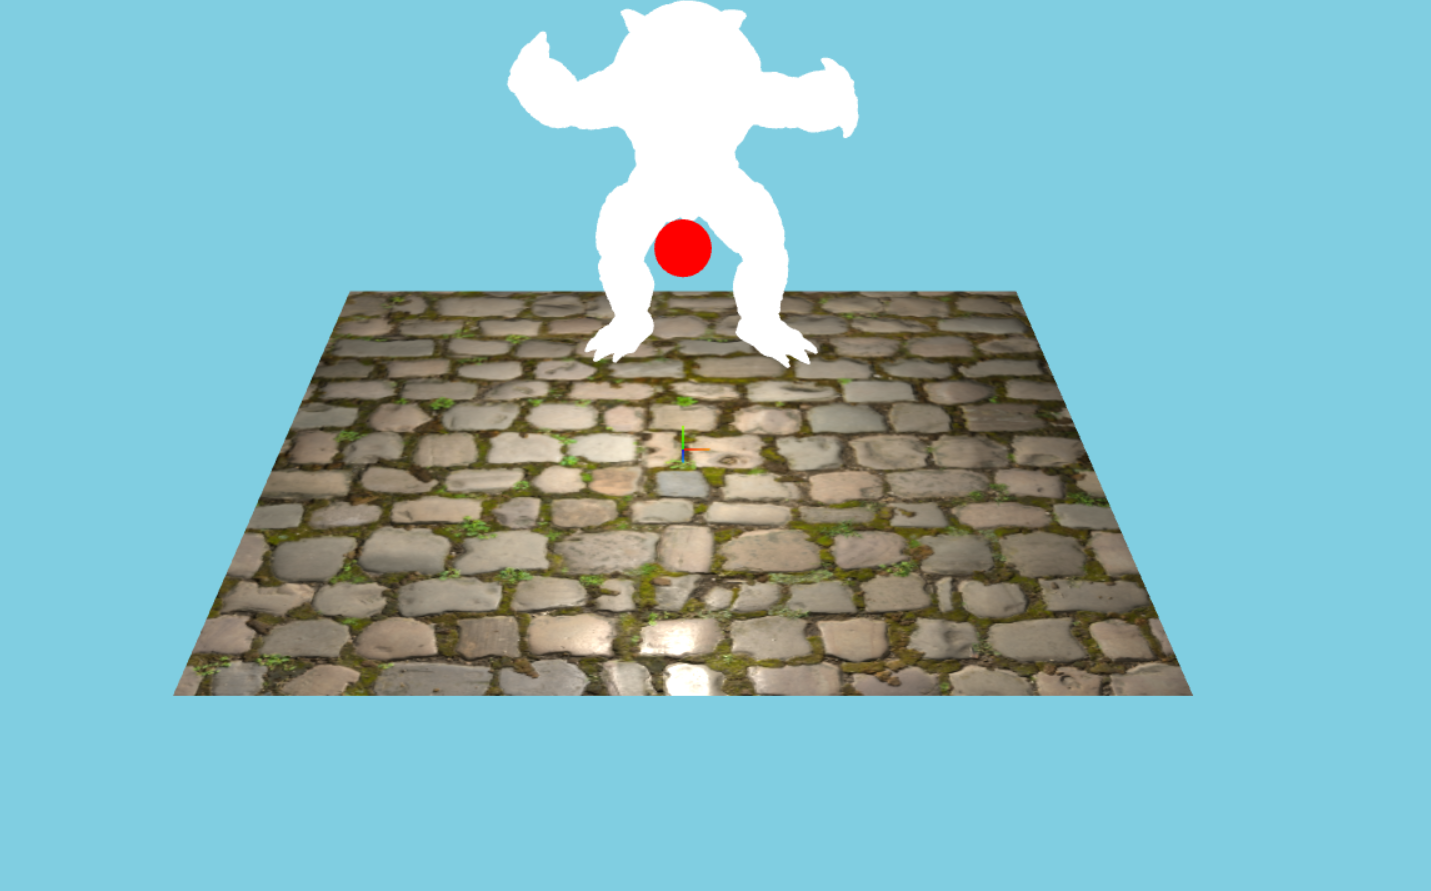
\includegraphics[width=0.4\textwidth]{./initial.png}
\end{figure}

{\bf Part 1: Required Elements}

\renewcommand{\labelenumi}{(\alph{enumi})}
\begin{enumerate}

\item {\bf 30 pts} Moving the Armadillo.

  Your goal for this part of the assignment is to get the Armadillo to respond to keyboard input. You have been given the coordinate frame of the armadillo as {\tt armadilloFrame}. You should manipulate this object, using the three.js API, to get the armadillo to slide forwards/backwards and side-to-side, you should also make the armadillo twirl in place. For the latter, the docs will likely be useful. \newline
  https://threejs.org/docs/\#api/en/core/Object3D.rotation
  
 \item {\bf 20 pts} Color the sphere with fragment normals.
 
 In this part, you need to color the sphere in its fragment shader {\tt sphere.fs.glsl} with fragment normals. In the vertex shader {\tt sphere.vs.glsl}, you can pass the attribute {\tt normal} to the fragment shader.  In the fragment shader, replace the RGB color using the fragment normal. This method is normally used to visualize the normal for debugging purposes.

 \begin{figure}[H]
  \centering
  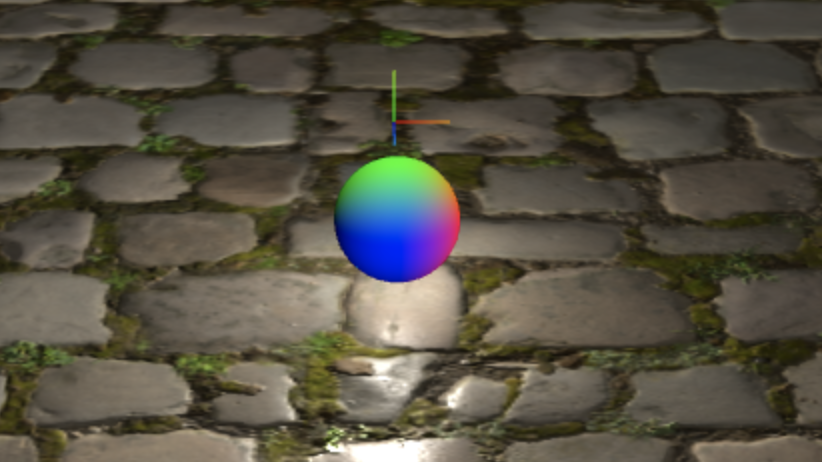
\includegraphics[width=0.4\textwidth]{./sphere.png}
\end{figure}

 \item {\bf 20 pts} Lighting the Armadillo.

  The light from the orb should light up the armadillo. Here you will
  implement a simple model of how light from the orb would interact
  with the armadillo, a simple shading model called ``Gouraud
  shading.''  We will study more realistic models later in the
  course. Modify {\tt A1.js} and {\tt armadillo.vs.glsl} to color each
  vertex of the armadillo based on the cosine of the angle between its
  normal and the direction vector to the center of the sphere. When
  correctly coded, the orb will be ``activated'', lighting up
  different parts of the armadillo as it's moved around, as
  illustrated in the figure below.

  \begin{figure}[H]
    \centering
    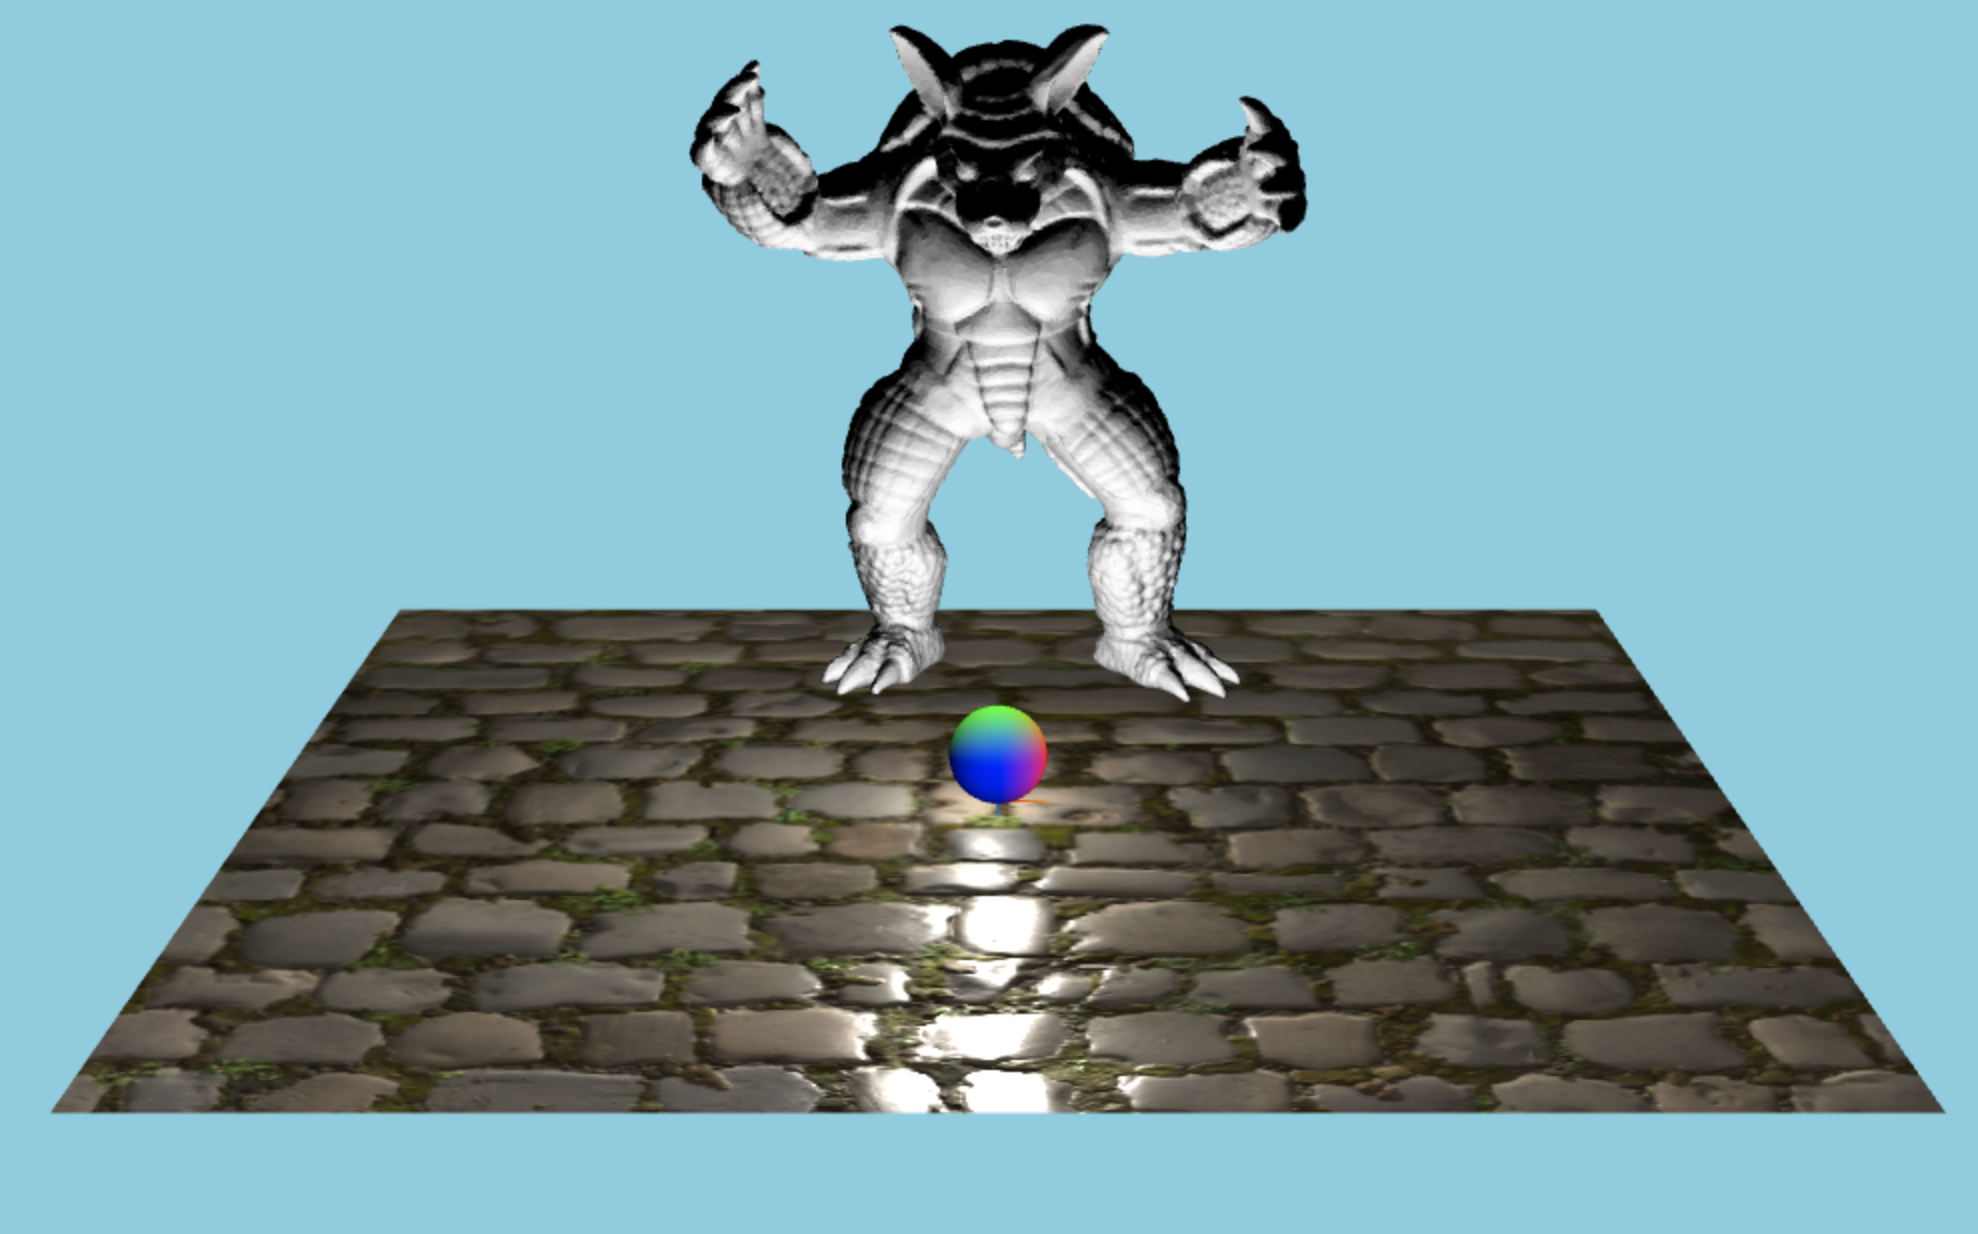
\includegraphics[width=0.4\textwidth]{./partC.png}
  \end{figure}

  \textit{Hint 1:} See how uniforms are passed to the sphere shader.

  \textit{Hint 2:} You should pass the necessary information about the sphere to the armadillo shaders.

  \textit{Hint 3:} See how varying variables are passed to the armadillo fragment shader.

\item {\bf 30 pts} Proximity detection.

 The armadillo has sensors on its skin that can detect objects in close proximity.
 For this part you will need to modify {\tt armadillo.fs.glsl} to further color the armadillo
 fragments green when in close proximity to the sphere, as illustrated in the figures
 below. One simple way is to check if an armadillo fragment is within a specified distance to the
 sphere, and if it is, set its color to green. 

\begin{figure}[H]
  \centering
  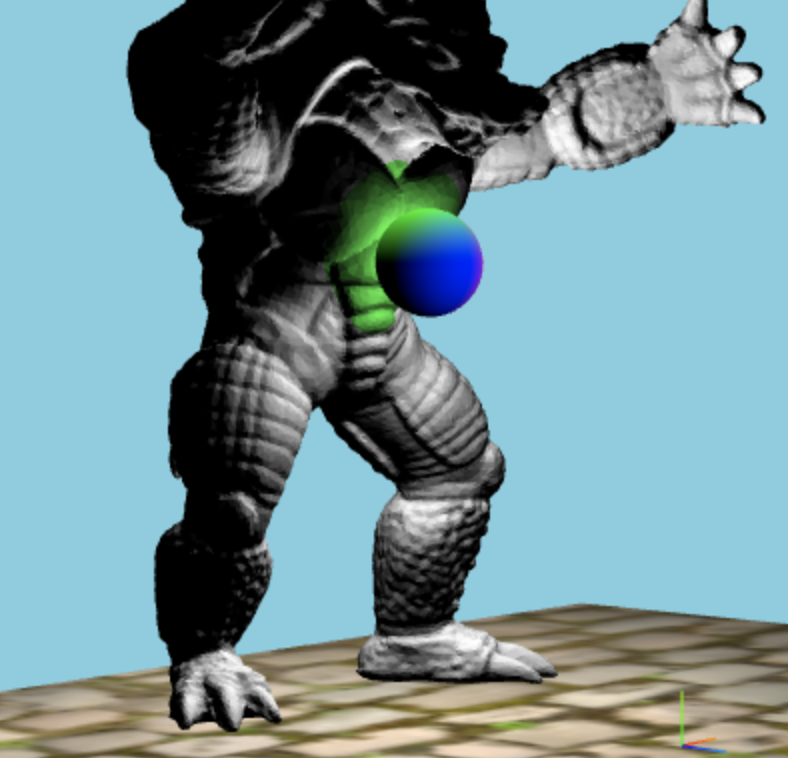
\includegraphics[width=0.4\textwidth]{./proximity.png}
\end{figure}

\textit{Hint:} You should use the appropriate uniform variable in the armadillo shader.
% \textit{Hint 2:} You may use one of the predefined transformation matrices, listed below.

% \medskip
% {\tt uniform mat4 modelMatrix;\\
% uniform mat4 modelViewMatrix;\\
% uniform mat4 projectionMatrix;\\
% uniform mat4 viewMatrix;\\
% uniform mat3 normalMatrix;}


% \item {\bf 30 pts} in 

%   Assemble the fancy Coronaorb. The real
%   coronaorb is decorated with multiple ``spikes.''  In this part you
%   will assemble the spikes on the spherical orb body, and make the
%   spikes move with the sphere. You will modify {\tt A1.js} to attach a
%   number of spikes to the sphere to form a realistic looking orb.  A
%   function called {\tt generateSphereSampling}, located in
%   `js/setup.js', is provided to help you position each instanced spike
%   around the sphere. Study the code used for adding the spike to the
%   scene and replace the provided transforms with transforms generated
%   by {\tt generateSphereSampling}.  You will also have to modify the spike
%   vertex shader (in {\tt spike.vs.glsl}) to move the spikes with the
%   orb, using the {\tt orbPosition} uniform.

% \begin{figure}[H]
%   \centering
%   \includegraphics[width=0.2\textwidth]{./final.png}
% \end{figure}


% \item {\bf 30 pts} Body Deformation.  

%   In this part you will indent the armadillo's mesh when pushed in by
%   the Orb, as illustrated in the figure below. This is a preview of
%   how vertex shaders can be used for changing a shape. For this you will
%   need to change {\tt armadillo.vs.glsl} and {\tt A1.js}. One simple
%   way is to check if a vertex is within the Orb, and if it is, move
%   the vertex to the surface. You should pass the necessary information
%   about the Orb to the armadillo shader.
% \begin{figure}[h]
%   \centering
%   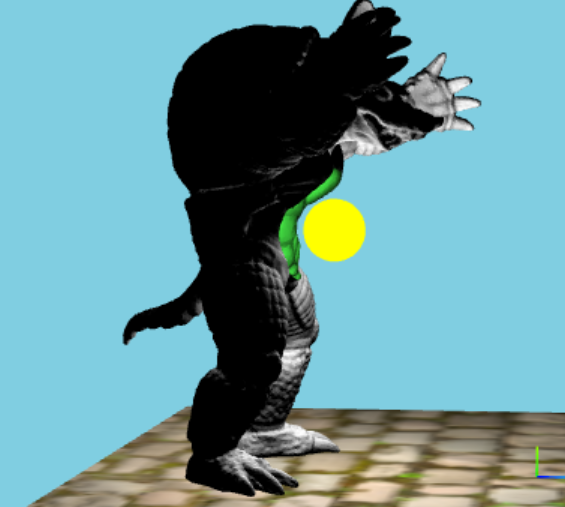
\includegraphics[width=0.4\textwidth]{./deformed.png}
% \end{figure}

% \textit{Hint 1:} See how uniforms are passed on the sphere
% shaders.
  
\end{enumerate}


{\bf Part 2: Creative License (Optional)}

You have many opportunities to unleash your creativity in
computer graphics!  In this \textbf{optional} section, and you are
invited to extend the assignment in fun and creative ways.
We'll highlight some of the best work in class. A small number of
exceptional contributions may be awarded bonus points.
Some possible suggestions might be:
\begin{itemize}
\item turn the Orb into a Coronavirus... very topical.
\item explode the armadillo or orb along face normals.
\item animate colors, lights, in fun ways. 
\item add interesting objects to the scene.
\end{itemize}


\section{Submission Instructions}
\subsection{Directory Structure}
Under the root directory of your assignment, create two subdirectories
named ``part1'' and ``part2'', and put all the source files, your
makefile, and everything else required to run each part in the respective
folder. Do not create more sub-directories than the ones already provided. 

You must also write a clear README.txt file that includes your name,
student number, and CWL username, instructions on how to use the
program (keyboard actions, etc.) and any information you would like to
pass on to the marker. Place README.txt under the root directory of your
assigment.

\subsection{Submission Methods}
Please compress everything under the root directory of your assignment into
{\tt a1.zip} and submit it on Canvas. You can make multiple submissions,
but we will grade only the last one.

\section{Grading}
\subsection{Point Allocation}
Each assignment has 100 points for Part 1. Part 2 is optional and you can get bonus points (0-10 points) at the
instruction team's discretion.
Percentage wise, we use Part 1's total points as the denominator: e.g. if you
get 95 out of 100 points from Part 1, but no points from Part 2, then your percentage
grade would be 95/100. If you get full points from both Parts, then your percentage
grade would be 110/100.

\subsection{Face-to-face (F2F) Grading}
For each assignment, you are required to meet face-to-face with a TA on Zoom or in person
to demonstrate that you understand why your program works. Details regarding how to
sign up a grading session with a TA will be announced on Canvas and on Piazza.

\subsection{Penalties}
Aside from penalties from incorrect solution or plagiarism, we may apply the following
penalties to each assignment:

\textbf{Late penalty.} You are entitled up to three grace (calendar) days in total
throughout the term. No penalties would be applied for using them. However once
you have used up the grace days, a deduction of 10 points would be applied to each
extra late day. Note that
\begin{enumerate}
  \item The three grace days are given for all assignments, \textbf{not per assignment}, so please use them wisely;
  \item We consider the time of only your last submission;
  \item We do not consider Part 1 and Part 2 submissions separately. Say if you submitted Part 1 on time but updated your submission for Part 2 one day after the deadline, we would count one late day.
\end{enumerate}

\textbf{No-show penalty.} You are required to sign up a grading slot at least one day
before F2F grading starts, and show up at your slot on time. So a 10-point deduction would
be applied to each of the following circumstances:
\begin{enumerate}
  \item Not signing up a grading slot before the sign-up period closes;
  \item Not showing up at your grading slot.
\end{enumerate}
Note that we would not apply the penalty if you are unable to sign up/show up on time
due to an emergency, or if you cannot sign up because none of the slots work for you.
In those cases, please contact the course staff immediately on Piazza.

\end{document}
%%% Local Variables:
%%% mode: latex
%%% TeX-master: t
%%% End:
